\documentclass[11pt]{article} \usepackage[margin=1in]{geometry}
\usepackage[T1]{fontenc} \usepackage[utf8]{inputenc} \usepackage{lmodern}
\usepackage{array} \usepackage{booktabs} \usepackage{enumitem}
\usepackage{setspace} \usepackage{titlesec}
\usepackage{tikz}
\usetikzlibrary{arrows.meta,positioning}

\setlength{\parindent}{0pt} \setlength{\parskip}{0.35em}
\setlist[itemize]{leftmargin=1.5em, itemsep=0.2em, topsep=0.2em}
\titleformat{\section}{\normalfont\bfseries}{\thesection.}{0.5em}{}
\titleformat{\subsection}{\normalfont\bfseries}{\thesubsection.}{0.5em}{}

% Title-page fields
\newcommand{\ProjectTitle}{GENESIS-AGENT: Generative Engine for Novel,
Explainable, Secure, and Integrated Simulation with Agentic Guidance, Execution,
and Reasoning} \newcommand{\LeadInstitution}{Sandia National Laboratories}
\newcommand{\StreetAddress}{TBD} \newcommand{\PostalAddress}{TBD}
\newcommand{\LeadPI}{TBD} \newcommand{\LeadPIContact}{TBD}
\newcommand{\AdminPOC}{TBD} \newcommand{\AdminPOCContact}{TBD}
\newcommand{\RFANumber}{DE-FOA-0003612} \newcommand{\PrimaryChallenge}{19 -- AI
for Scientific Reasoning} \newcommand{\PrimaryFocusArea}{A/B/C -- Trustworthy
Mathematical and Symbolic Reasoning; Hypothesis Generation from Multi-Modal
Data; Composable and Modular Foundation Models}
\usepackage{comment}
\begin{document}

\pagenumbering{gobble} \begin{titlepage} \thispagestyle{empty} \begin{center}
{\Large \textbf{\ProjectTitle}\par} \end{center}

\vspace{1em} \textbf{Lead Applicant/Institution:} \LeadInstitution

\textbf{Street Address:} \StreetAddress

\textbf{Postal Address:} \PostalAddress

\textbf{Lead PI name, telephone number, email:} \LeadPI; \LeadPIContact

\textbf{Administrative Point of Contact name, telephone number, email:}
\AdminPOC; \AdminPOCContact

\textbf{RFA Number:} \RFANumber

\textbf{Primary challenge and focus area:} \PrimaryChallenge{} $|$
\PrimaryFocusArea

\vspace{1em} \textbf{Senior/Key Personnel for Lead Institution and All Partner
Institutions}

\begin{tabular}{p{0.35\textwidth} p{0.6\textwidth}} \toprule \textbf{Institution
Name} & \textbf{Senior/Key Personnel including the Director} \\ \midrule
\LeadInstitution{} (Lead) & TBD \\ Partner Institution 1 & TBD \\ Partner
Institution 2 & TBD \\ \bottomrule \end{tabular}

\vspace{1em} \textbf{Summary budget information for lead institution and all
partner institutions}

\begin{tabular}{p{0.65\textwidth} p{0.25\textwidth}} \toprule
\textbf{Institution} & \textbf{Year 1 Budget \$} \\ \midrule \LeadInstitution{}
(Lead) & TBD \\ Partner Institution 1 & TBD \\ Partner Institution 2 & TBD \\
\textbf{Total} & TBD \\ \bottomrule \end{tabular} \end{titlepage}

\clearpage \pagenumbering{arabic}


\begin{comment}
\section{Executive summary} In this Phase-1 proposal, we propose to develop the
first stage of an agentic AI platform capable of automating the
hypothesis-to-response workflow within the DoE enterprise. Broadly, we envision
a platform enabling multi-agent workflows capable of synthesizing scientific
information, formulating research questions, orchestrating outer-loop analyses
through established DOE codes (e.g., uncertainty quantification through Dakota),
setting up and formulating inner-loop model evaluation (with tasks including
meshing, input-deck generation, model execution in HPC environments),
goal-oriented post-processing, and hypothesis refinement. In Phase 1, we will
consider a subset of this goal: orchestrationg outer-loop analyses through
established DoE codes, managing inner loop model evaluations (including input
deck generation and model execution, but restricting mesh generation), and and
goal-oriented postprocessing. We will achieve this goal through a coordinated
multiagent workflow working within a Model Context Protocol (MCP) interface. MCP
will be used to homogonize the toolcalling, model execution, and 
\end{comment}

\section{Background/Introduction} Agentic
artificial intelligence (AI) is poised to transform analysis and
hypothesis-driven computational science workflows within DOE.
Traditionally, these pipelines have depended on
scientists and engineers translating hypotheses into end-to-end computational
studies, from which conclusions can be drawn. This process involves designing outer-loop analyses (e.g.,
optimization and uncertainty quantification), constructing computational
experiments (which can involve formulating an outer-loop analysis, meshing, configuring and executing large-scale simulation codes,
and post-processing quantities of interest), and iteratively refining subsequent
experiments. The dominant bottleneck in this process is not computational cost,
but the substantial human effort required to generate, execute, and monitor this
pipeline.

Recent advances in agentic AI are beginning to shift this paradigm. Commercial
systems such as Claude, Codex, and Cursor—paired with frontier large language
models (LLMs)—enable users to orchestrate complex workflows, autonomously
analyze results, and respond to sophisticated scientific queries. While these
capabilities have primarily emerged within coding environments, the underlying
LLMs and agentic technologies show strong promise for more ambitious scientific workflows
and underpin emerging concepts such as the ``AI Scientist.'' This shift is
already underway in aspects of the community, were AI-driven workflows have
emerged for, e.g., computational fluid dynamics workflows~\cite{},
finite element analysis workflows~\cite{}, materials design, the solution of
mechanical probelms, and others. These developments
highlight a pathway toward autonomous, AI-driven research and analysis and
present a transformative opportunity for the DOE enterprise. 

Realizing this vision within DOE, however, requires significant advances. We
highlight several key challenges:

\begin{itemize} \item \textbf{Heterogeneity of workflows and codes.} Existing
agentic systems have demonstrated success in constrained environments with
narrowly defined objectives. In contrast, DOE workflows are often extensive,
requiring subject matter expertise across multiple domains. These workflows often begin with abstract hypothesis generation, proceeding
through multi-stage computational studies across diverse simulation codes, and
oftentimes culminating in complex, large-scale data analysis. The entry points
for workflows are often distnict as well: some workflows require simple
execution of a parameter study, while some involve creating a hypothesis and
designing subsequent experiments to assess this hypothesis. Regardless,
workflows within DOE require use of a myriad of physics and analysis codebases, and each codebase
introduces distinct requirements for e.g., input specifications, problem
formulation, meshing, execution environments, and typically requires oversight from a
subject-matter expert to ensure reliable simulations. Effective use of these
tools also requires detailed knowledge of HPC systems, including scheduling,
resource availability, and data management. Compounding this challenge, many DOE
codes are proprietary and absent from standard LLM training data. 

Enabling agentic workflows in this complex setting requires new approaches to
scale agentic workflows and synthesize diverse domain knowledge, toolkits, and operating
environments into structured representations that AI systems can reliably
execute.

\item \textbf{Validation and trust.} Scientific applications within DOE are
often high-consequence, where incorrect conclusions can lead to significant
downstream impacts. While agentic AI systems are powerful, they are not
infallible. It is widely established that, while the power of agentic
technologies has become accepeted, there remains a trust gap between many
developers and users. Thus, to be a reliable tool for DOE analyses, we require
the development of frameworks that provide rigorous validation, uncertainty quantification, self-audit capabilities, and
mechanisms for human-in-the-loop oversight when needed.

    \item \textbf{Security and operational constraints.} Agentic AI systems
within DOE must operate under substantially stricter security requirements than
those in commercial or academic environments. These include constraints on data
movement, the need for on-premises or air-gapped LLM deployments, and careful
management of interactions between agents and external tools. In particular,
reliance on off-premises frontier models and commercial software introduces
risks related to data exposure and reduced visibility and control over data and
execution pathways. Ensuring secure operation requires robust sandboxing,
fine-grained access control, and verifiable policies governing tool use and
system interactions.  \end{itemize}

\section{Project Objectives}
This Phase I effort will deliver the core framework elements needed to achieve
AI advantage for simulation-centric scientific workflows in DOE environments.
The project objective is to build and evaluate a prototype software framework
that combines structured workflow representations, retrieval-grounded
reasoning, tool execution, and human-in-the-loop review so that agents can
assist with planning, executing, and refining computational studies across
heterogeneous DOE codes.

The specific Phase I objectives are:
\begin{itemize}
\item Define a structured workflow framework that represents user intent,
required files, dependencies, validation checks, tool invocations, and review
gates in a form that agents can reason over and execute reliably.
\item Separate the front-end orchestration layer from the back-end model layer
so the framework can securely adopt different approved LLMs as deployment
policy allows.
\item Build framework services for dependency-aware generation and validation of
auditable input decks and for execution of representative downstream analysis
workflows.
\item Demonstrate secure, open-source, on-premises deployment with policy
enforcement, human-in-the-loop review, and adaptable open-weight models.
\item Package orchestration, tool-integration, provenance, and deployment
infrastructure so it can be transferred across DOE programs, codes, and
security environments.
\end{itemize}

These objectives align directly with the chosen focus topic, \textit{AI for
Scientific Reasoning}. GENESIS-AGENT is not limited to summarization or
autocomplete; it is designed to reason across natural-language objectives,
structured workflow specifications, scientific software interfaces, execution
logs, and simulation outputs. By integrating model reasoning with formal
workflow representations, retrieval, and controlled tool use, the project
targets trustworthy mathematical and symbolic reasoning, multi-modal scientific
context, and composable AI system design.

The proposed objectives lead to AI advantage by reducing the human effort
required to formulate, validate, execute, and refine computational studies.
Instead of requiring users to manually translate intent into code-specific
inputs and execution steps, the framework will provide reusable agentic
infrastructure that accelerates workflow setup, improves consistency and
auditability, and enables secure adoption across evolving DOE modeling and
simulation environments.

\section*{Proposed work: GENESIS-AGENT}
To address these challenges, we propose \textbf{GENESIS-AGENT}, a
\textbf{G}enerative \textbf{E}ngine for \textbf{N}ovel, \textbf{E}xplainable,
\textbf{S}ecure, and \textbf{I}ntegrated \textbf{S}imulation with Agentic
AI, designed for deployment within the DOE ecosystem. Our long-term vision is
to develop an AI system capable of operating at the level of a postdoctoral
researcher. Under human oversight, the agent will synthesize scientific
knowledge, formulate and refine hypotheses, orchestrate computational analyses
using established DOE tools (including outer-loop workflow generation,
meshing, input-deck construction, and HPC execution), and iteratively improve
through interaction with a human advisor. We explicitly distinguish this effort from existing approaches, such as the
AI Scientist, which aim to develop fully autonomous agentic workflows for
science. We contend that full autonomy is the incorrect paradigm for DOE modeling and
simulation. Instead, we focus on a human-in-the-loop approach that more closely
reflects how computational science is conducted. In practice, progress in
modeling and simulation comes from iteration, discussion, and validation across
teams - not from a single fully autonomous process. We view agentic AI systems in
the same way: as collaborators rather than replacements. By integrating human
feedback directly into the workflow, GENESIS-AGENT is designed to produce
results that are more reliable, interpretable, and ultimately more useful for
scientific discovery.
  
To achieve this goal, we propose to design GENESIS-AGENT as a multi-agent
system comprising three layers: (1)
an \textbf{agent layer}, (2) an \textbf{MCP/tooling layer}, and an (3) \textbf{LLM
layer}. The agent layer comprises a hierarchical suite of Python-based agents, ranging
from scientific reasoning agents to code-specific agents tailored to simulation
tools. These agents are responsible for workflow planning and orchestration,
input-deck generation, code execution,
validation, and downstream analysis. These agents will incorporate retrieval augmented
generation (RAG) pipelines tailored to DOE applications so they can access
specialized documentation, prior workflows, and other domain context at
inference time. Second, we will develop MCP layers to provide
standardized interfaces for workflow tools that are going to be reusable by
different codes, different agents, and different parts of the workflow. Examples
include services such as job submission, monitoring, and data management across
HPC systems. Lastly, the LLM layer, which provides the underlying reasoning
techologies, will be designed to be backend-agnostic,
enabling seamless integration with frontier commercial models, locally hosted
models, or on-premises deployments. This layered architecture provides both
flexibility and security, enabling robust, scalable, and trustworthy agentic
workflows within DOE. 

Across all of the above areas, we will focus on the development of methodologies
that are scalable, secure, and can be validated.
  

In developing GENESIS-AGENT, we will address the following research quesetions:
\begin{itemize}
\item How to develop an agentic AI system which can scale to a diverse ecosystem
of codes, analysis tools, and execution environments.
\item How to ensure verifiability of agent-produced product.
\item Effecitely developing a framework with multiple entry points.
\end{itemize}

The following section provides a more detailed description of the proposed
design and research.
%At the highest level, a \textit{research agent} will be capable of
%working, with human oversite, to parse literature and develop novel research
%hypotheses and tasks. At the next level, a \textit{planning agent} will
%interpret the output of the research agent, decompose the hypothesis into a
%series of tasks, and coordinate subsequent downstream actions. This planner interfaces with a collection of \emph{specialized agents},
%including code-specific agents tailored to individual simulation tools (e.g.,
%Sierra/Aria, SPARC, Dakota) and \textit{execution agents} tailored to submitting
%and managing HPC jobs in the DOE ecosystem. These code-specific agents encapsulate detailed
%knowledge of input-deck construction, meshing strategies, solver configurations,
%execution workflows, and post-processing routines, while the execution agents
%retain detailed knowledge about HPC environments, resource availibility, job
%submission, etc. 
 
%including code-specific agents tailored to individual simulation tools that
%handle input generation, execution, validation, and analysis. 
\subsection*{System Architecture}
We design GENESIS-AGENT as a three-layered system consisting of: (1) an
\textbf{agent layer}, (2) an \textbf{MCP/tooling layer}, and (3) an \textbf{LLM
layer}. This decomposition separates reasoning, execution, and model inference,
enabling modularity, scalability, and secure deployment.

\begin{figure}[t]
\centering
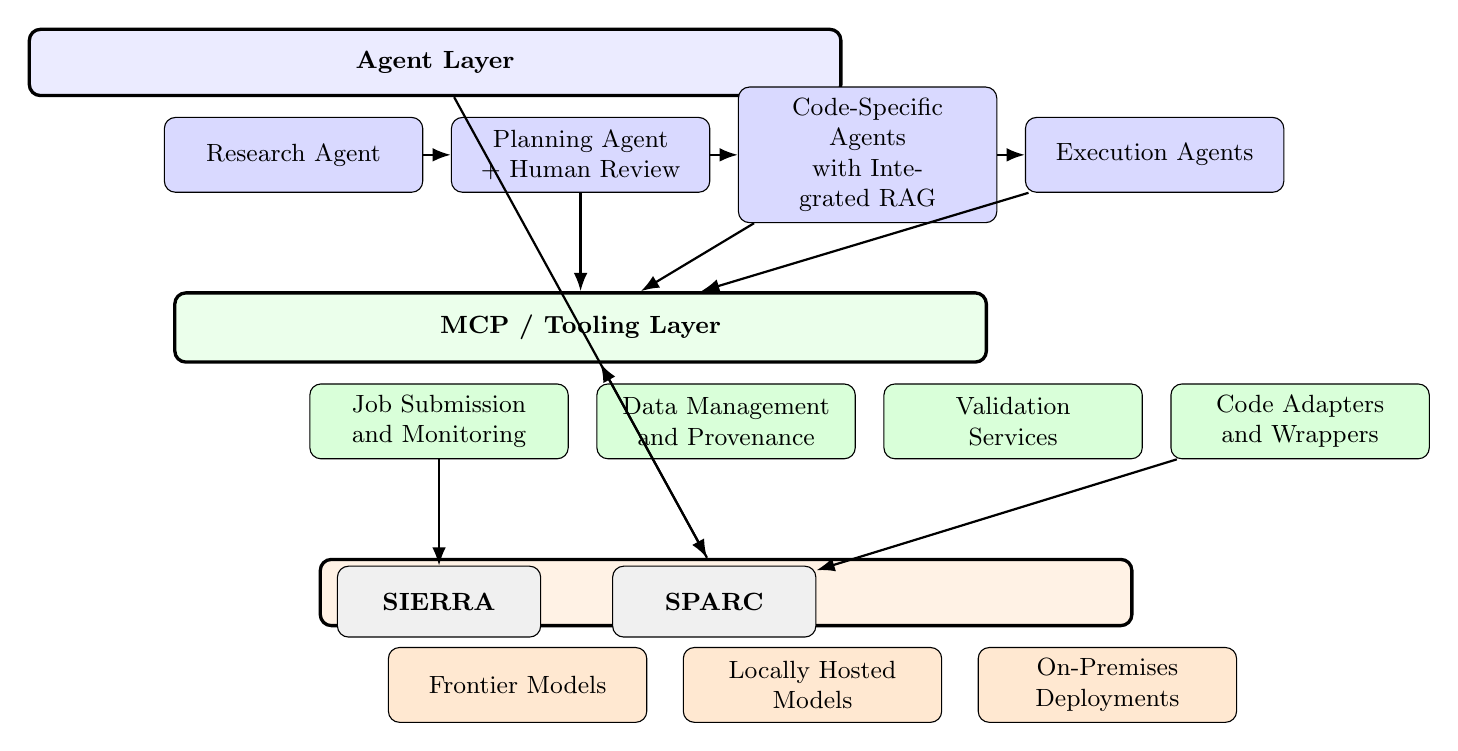
\begin{tikzpicture}[
  font=\small,
  >=Latex,
  node distance=0.45cm and 0.55cm,
  layer/.style={draw, rounded corners, very thick, minimum width=0.85\textwidth, align=center, inner sep=8pt},
  box/.style={draw, rounded corners, align=center, minimum height=0.95cm, text width=3.0cm, inner sep=4pt},
  codebox/.style={draw, rounded corners, align=center, minimum height=0.9cm, text width=2.3cm, inner sep=4pt},
  flow/.style={->, thick}
]
\node[layer, fill=blue!8] (agent) {\textbf{Agent Layer}};
\node[box, fill=blue!15, below left=0.25cm and 0.15cm of agent.south] (research) {Research Agent};
\node[box, fill=blue!15, right=0.35cm of research] (planner) {Planning Agent\\+ Human Review};
\node[box, fill=blue!15, right=0.35cm of planner] (codeagents) {Code-Specific Agents\\with Integrated RAG};
\node[box, fill=blue!15, right=0.35cm of codeagents] (exec) {Execution Agents};

\node[layer, fill=green!8, below=1.25cm of planner] (mcp) {\textbf{MCP / Tooling Layer}};
\node[box, fill=green!15, below left=0.25cm and 0.15cm of mcp.south] (jobs) {Job Submission\\and Monitoring};
\node[box, fill=green!15, right=0.35cm of jobs] (data) {Data Management\\and Provenance};
\node[box, fill=green!15, right=0.35cm of data] (validate) {Validation\\Services};
\node[box, fill=green!15, right=0.35cm of validate] (adapters) {Code Adapters\\and Wrappers};

\node[layer, fill=orange!10, below=1.25cm of data] (llm) {\textbf{LLM Layer}};
\node[box, fill=orange!18, below left=0.25cm and 1.0cm of llm.south] (frontier) {Frontier Models};
\node[box, fill=orange!18, right=0.45cm of frontier] (local) {Locally Hosted\\Models};
\node[box, fill=orange!18, right=0.45cm of local] (prem) {On-Premises\\Deployments};

\node[codebox, fill=gray!12, below=1.35cm of jobs] (sierra) {\textbf{SIERRA}};
\node[codebox, fill=gray!12, right=0.9cm of sierra] (sparc) {\textbf{SPARC}};

\draw[flow] (research) -- (planner);
\draw[flow] (planner) -- (codeagents);
\draw[flow] (codeagents) -- (exec);

\draw[flow] (planner) -- (mcp);
\draw[flow] (codeagents) -- (mcp);
\draw[flow] (exec) -- (mcp);

\draw[flow] (agent) -- (llm);
\draw[flow] (jobs) -- (sierra);
\draw[flow] (adapters) -- (sparc);
\draw[flow] (llm) -- (mcp);
\end{tikzpicture}
\caption{Proposed GENESIS-AGENT architecture. A hierarchical agent layer performs planning, code-specific reasoning, and execution management, with retrieval integrated into the code-specific agents. Shared MCP services mediate workflow execution and connect the agent stack to target simulation codes including SIERRA and SPARC, while the backend LLM layer remains deployment-agnostic.}
\label{fig:genesis-architecture}
\end{figure}


\paragraph{Agent Layer.} The agent layer comprises a hierarchical suite of
Python-based agents responsible for scientific reasoning and workflow
orchestration. At the highest level, a \textit{research agent} will be capable of
working, with human oversite, to parse literature and develop novel research
hypotheses and tasks. At the next level, a \textit{planning agent} will
interpret the output of the research agent, decompose the hypothesis into a
series of tasks, and coordinate subsequent downstream actions. Inspired by
recent ideas within agentic coding tools, we propose to create the planning
agent to support \textit{human-in-the-loop} interactions. In this setting, the planning agent
will create the initial plan, propose it to a human reviewer, who will then
approve or ierate the plan. Once finalized, the planner interfaces with a collection of \emph{specialized agents},
including code-specific agents tailored to individual simulation tools (e.g.,
Sierra/Aria, SPARC, Dakota) and \textit{execution agents} tailored to submitting
and managing HPC jobs in the DOE ecosystem. These code-specific agents encapsulate detailed
knowledge of input-deck construction, meshing strategies, solver configurations,
execution workflows, and post-processing routines, while the execution agents
retain detailed knowledge about HPC environments, resource availibility, job
submission, etc. Initially, these tailored agents will be constructed through feature engineering
and agent design tailored to specific codebases and tasks. Rather than pursuing MCP at the fine-grained code level, we will
instead develop task-specific agents with complete knowledge of how to execute
the simulation workflow. To help these agents navigate DOE's complex
computational ecosystem, we will embed retrieval augmented generation (RAG)
capabilities directly into the agent layer. Initially, we propose to develop
tool-specific retrieval pipelines that treat documentation, prior workflows,
and validated inputs as retrievable knowledge sources at inference time. To
effectively manage multimodal information, these agent-facing retrieval
pipelines will leverage hybrid search strategies, combining similarity searches
on embeddings with keyword matching and metadata constraints to identify
relevant context.
 

\paragraph{MCP Layer}
Second, we will develop MCP layers to provides
standardized interfaces for workflow tools that are reusable by
different codes, different agents, and different parts of the workflow. Examples
include services such as job submission, monitoring, and data management across
HPC systems. This abstraction will be critical to enabling a scalable agentic
system that can work across the diverse environments encountered within DOE.
A critical question we will address in the development of MCP interfaces is
 what level of abstraction these interfaces should be placed at. For
instance, specific MCP interfaces could be placed within a simulation-level
context, e.g., creating solver portions of an input deck, creating boundary
conditions, etc. As these interfaces become more fine-grained, the overall
framework may become too brittle. The development of MCPs at too coarse-grained
of a level, however, will mitigate their ability to be re-used.


\paragraph{LLM layers}
Lastly, the LLM layers provides the underlying reasoning capabilities to the
system. Critically, we will design GENESIS-AGENT such that the LLM layers are backend-agnostic,
enabling seamless integration with frontier commercial models, locally hosted
models, or on-premises deployments. This layered architecture provides both
flexibility and security, enabling robust, scalable, and trustworthy agentic
workflows within DOE. Furthermore, it allows GENESIS-AGENT to support fine-tuned
models calibrated to each task. Within Sandia, we will specifically focus on integration
with Shirty Microservices, which hosts on-prem open-source LLMs and is an
underlying technology of initial efforts to provide enterprise-wide LLM access
on secure datasets and agentic
coding assistance.


\section*{Phase 1 deliverables}
Within Phase 1, we aim to deliver a minimum working example of the proposed
pipeline. Specifically, we will demonstrate an end-to-end agent-driven analysis
workflow in which agents formulate an outer-loop analysis plan, refine that plan
through human-in-the-loop review, execute the resulting workflow, including
input-deck generation, model execution, and post-processing, and return the
results to the user for further refinement. This demonstration will integrate at
least two candidate outer-loop analysis drivers and three physics codebases,
including two internal DOE codes and one external code. As candidate outerloop
analysis drivers, we will consider Dakota, PyTUK, and rom-tools-and-workflows.
As candidate DOE physics codebases, we will consider Sandia's Sierra/Aria (heat
transfer) and SPARC (fluid dynamics). As candidate open-souce codebases, we will
consider OpenFOAM, which is a widely used open-source computational fluid
dynamics code. 


 
\begin{comment}
\section*{Proposed Approach: GENESIS-AGENT}
To address these challenges, we propose \textbf{GENESIS-AGENT}—a
\textbf{G}enerative \textbf{E}ngine for \textbf{N}ovel, \textbf{E}xplainable,
\textbf{S}ecure, and \textbf{I}ntegrated \textbf{S}imulation with Agentic
AI—designed for deployment within the DOE ecosystem. Our long-term vision is to
develop an AI system capable of operating at the level of a postdoctoral
researcher: synthesizing scientific knowledge, formulating and refining
hypotheses, orchestrating computational campaigns, and iteratively improving
conclusions under human supervision. In this paradigm, the agent serves as an
intelligent outer-loop controller, coordinating complex simulation workflows
while maintaining alignment with scientific objectives, uncertainty
quantification requirements, and operational constraints.

Achieving this vision requires advances beyond current agentic systems,
particularly in enabling reliable reasoning over heterogeneous, domain-specific
workflows under strict security and validation constraints. The central research
challenge is therefore to develop methods for \emph{structured, verifiable, and
secure agentic reasoning} over DOE-scale simulation ecosystems. GENESIS-AGENT
addresses this challenge through a multilayered architecture that integrates
domain knowledge, workflow orchestration, and model reasoning in a principled
manner.

\subsection*{System Architecture}

We design GENESIS-AGENT as a three-layered system consisting of: (1) an
\textbf{agent layer}, (2) an \textbf{MCP/tooling layer}, and (3) an \textbf{LLM
layer}. This decomposition separates reasoning, execution, and model inference,
enabling modularity, scalability, and secure deployment.

\paragraph{Agent Layer.} The agent layer comprises a hierarchical suite of
Python-based agents responsible for scientific reasoning and workflow
orchestration. At the highest level, a \emph{planning agent} interprets
scientific objectives, decomposes tasks, and coordinates downstream actions.
This planner interfaces with a collection of \emph{specialized agents},
including code-specific agents tailored to individual simulation tools (e.g.,
Sierra/Aria, SPARC, Dakota). These code-specific agents encapsulate detailed
knowledge of input-deck construction, meshing strategies, solver configurations,
execution workflows, and post-processing routines.

A key design principle is that these agents operate over \emph{structured
representations} of the workflow rather than unstructured text alone. For
example, input decks are generated via intermediate schema-based representations
(e.g., typed JSON/YAML specifications of physics models, boundary conditions,
and solver parameters), which are then deterministically compiled into
code-specific formats. This approach improves reliability, reduces
hallucination, and enables explicit validation of intermediate states.

Agent interactions are further organized through a hierarchical control
structure, enabling decomposition of complex tasks into smaller, verifiable
subtasks (e.g., problem formulation, discretization, execution, analysis). This
design supports iterative refinement, where agents can propose candidate
workflows, validate outcomes, and adapt strategies based on feedback.

\paragraph{MCP/Tooling Layer.} The MCP (Model Context Protocol) layer provides
standardized, reusable interfaces to shared computational services. Rather than
embedding all functionality within individual agents, this layer exposes
capabilities such as: \begin{itemize} \item HPC job submission and scheduling
(e.g., SLURM interfaces), \item job monitoring and failure detection, \item
filesystem and data management, \item access to curated datasets, templates, and
prior simulation results, \item validation services (e.g., input-deck checking,
schema validation, and lightweight preflight simulations).  \end{itemize}

This abstraction enables separation of concerns between reasoning and execution,
allowing agents to focus on decision-making while delegating operational tasks
to controlled services. Importantly, the MCP layer provides a natural point for
enforcing \emph{security, access control, and auditing policies}, ensuring that
agent actions remain compliant with DOE requirements. By centralizing these
capabilities, MCP also promotes reuse across multiple agents and simulation
codes, reducing duplication and improving maintainability.

\paragraph{LLM Layer.} The LLM layer provides the underlying reasoning and
language capabilities for the system. GENESIS-AGENT is designed to be
\emph{backend-agnostic}, supporting integration with frontier commercial models,
locally hosted open-source models, and on-premises deployments. This flexibility
is critical for DOE environments, where security constraints may prohibit the
use of off-premises models.

To enable robust performance, the LLM layer is augmented with retrieval
mechanisms over domain-specific corpora, including documentation, prior
simulation campaigns, and validated input decks. Rather than relying solely on
pretrained knowledge, the system dynamically incorporates relevant context at
inference time, enabling adaptation to proprietary codes and evolving workflows.
\end{comment}


\subsection*{Key Technical Innovations}

GENESIS-AGENT introduces several key innovations necessary for reliable agentic
workflows in DOE environments:

\begin{itemize} \item \textbf{Structured workflow representations:} The use of
intermediate, schema-based representations enables verifiable reasoning and
deterministic compilation into simulation inputs.
    
    \item \textbf{Validation-aware agent design:} Agents are tightly coupled
with validation and repair loops, enabling iterative refinement through
automated checks, error parsing, and corrective actions.
    
    \item \textbf{Hybrid reasoning and execution:} The system integrates
LLM-based reasoning with deterministic tools and domain-specific rules, ensuring
that critical operations remain reliable and interpretable.
    
    \item \textbf{Secure and modular infrastructure:} The MCP layer enforces
controlled access to computational resources while enabling reuse and
interoperability across agents and codes.
    
    \item \textbf{Memory and experience reuse:} The system maintains a database
of prior simulation workflows and outcomes, enabling case-based reasoning and
transfer across related problems.  \end{itemize}

\subsection*{Deployment within DOE Ecosystems}

Within Sandia, we will integrate GENESIS-AGENT with Shifty Microservices, which
provide access to on-premises open-source LLMs and support emerging enterprise
agentic capabilities. This integration enables secure deployment while
maintaining compatibility with evolving DOE infrastructure.

\subsection*{Evaluation and Impact}

We will evaluate GENESIS-AGENT on representative DOE workflows, including
uncertainty quantification, inverse problems, and multiphysics simulation
campaigns. Key metrics will include: \begin{itemize} \item reduction in human
time required to configure and execute workflows, \item success rate of
automated input-deck generation and execution, \item robustness to workflow
complexity and heterogeneity, \item quality and reliability of scientific
outputs.  \end{itemize}

Ultimately, GENESIS-AGENT aims to transform the role of scientists and engineers
from manual workflow execution to high-level scientific reasoning, enabling
faster, more reliable, and more scalable discovery within the DOE enterprise.





To ensure modularity and interoperability, we will develop Model Context
Protocol (MCP) servers for each target simulation capability (e.g., Sandia’s
Sierra codes and Dakota workflows). Each MCP server will expose a well-defined
interface for a specific task (e.g., simulation execution or UQ orchestration)
while internally coordinating an agentic workflow to satisfy code-specific input
requirements. For example, a simulation execution MCP will encapsulate the
end-to-end process of constructing a valid input deck, submitting jobs to DOE
HPC systems, monitoring execution, and returning structured outputs. By
combining these MCP-backed capabilities with higher-level task agents,
GENESIS-AGENT will enable composable, reliable workflow automation, while
maintaining transparency and control over each stage of the simulation pipeline.

%Starting with each target simulation code, we wil develop MCPs ensuring
%interpoability. Each one of these MCPs will internaly orchastrate an agentic
%workflow to achieve a specific task. As a concrete example, a simulation agent
%will be response  
%
%we will develop structured simulation interfaces and constraint-aware planning
%mechanisms that enable agents to reason over feasible actions, rather than
%relying on unconstrained text generation. 
 

 
 


We propose a GENESIS-AGENT, a \textbf{G}enerative \textbf{E}ngine for
\textbf{N}ovel, \textbf{E}xplainable, \textbf{S}ecure, and \textbf{I}ntegrated
\textbf{S}imulation with Agentic Guidance, Execution, and Reasoning. Scientific
progress within the DOE enterprise depends on the ability of scientists and
engineers to translate hypotheses into executable computational studies, run
those studies at scale, interpret the results, and refine the next experiment.
In practice, this process 

, the burden of generating and validating input decks, and the expertise
required to connect simulation codes to downstream analysis workflows. Agentic
AI has created a credible path toward a step change in this workflow by moving
beyond question answering to planning, tool use, execution, and iterative
refinement.

That opportunity is coupled to a strategic risk. If DOE workflows are built
primarily around commercial closed models and proprietary agent platforms, then
DOE inherits toolchain dependence on external vendors whose access policies,
business incentives, and deployment constraints are outside DOE control. Equally
important, agentic systems expand the cyber and operational attack surface
because they retrieve data, invoke tools, modify files, and launch actions. It
is also not realistic for a Phase I DOE effort to recreate a full vertically
integrated frontier-agent stack from scratch. The practical path for DOE is
instead to build the framework layer that DOE must own regardless of which
models are used: structured workflow representations, validation and policy
engines, tool adapters, provenance, secure execution, and modular deployment
interfaces.

We propose to address this gap through GENESIS-AGENT, an open, on-premises
framework for agentic scientific workflows. The primary deliverable is a
reusable software framework that lets DOE teams define structured task
specifications, generate and validate code-specific inputs, execute workflows
through policy-aware tool wrappers, capture provenance, and connect approved
language models through a stable interface.

A defining principle of GENESIS-AGENT is modularity across both the front-end
orchestration layer and the back-end model layer. The front end will provide the
framework capabilities needed for planning, retrieval, tool selection, execution
monitoring, provenance tracking, human review, and policy enforcement. The back
end will expose interchangeable model interfaces so that the same orchestration
stack can work with different open-weight LLMs, frontier models, or specialized
scientific models as institutional security policy permits. This separation is
essential for DOE deployment because it allows the framework, tool adapters, and
governance mechanisms to remain stable even as model technology evolves or as
security constraints require a transition between model providers, hosting
modes, or classification boundaries.

The proposed effort directly addresses Challenge 19, AI for Scientific
Reasoning, because the system is not merely intended to summarize or
autocomplete. It will reason across natural-language requirements, structured
input specifications, scientific software interfaces, execution logs, and
analysis outputs. By integrating LLM-based reasoning with formal workflow
representations and external tools, the system will help formulate a
computational experiment, instantiate it in code-specific form, run it, evaluate
outcomes, and recommend refinements.

This project is especially well aligned with Sandia and the DOE mission. By
delivering a secure, modular framework for workflow specification, validation,
execution, and adaptation, we can reduce time-to-study, lower the barrier to
advanced computational methods, and create reusable infrastructure for agentic
scientific workflows throughout DOE. Representative application targets include
input-deck generation, parameter studies, and reduced-order modeling pipelines.

\textbf{Infrastructure statement:} The proposed project does not involve the
construction, alteration, maintenance, or repair of public infrastructure in the
United States.

\section{Proposed Research and Methods} Our central hypothesis is that robust
scientific workflow reasoning emerges from a composable framework rather than
from a single monolithic model. To test this, we will implement a prototype
orchestration architecture that turns user requests into structured workflow
objects, routes those objects through validation and generation services,
executes approved tools, and records the resulting artifacts and decisions.

The architecture will be explicitly split into a front-end orchestration plane
and a back-end model plane. The front-end plane will manage planning, retrieval,
tool invocation, policy enforcement, logging, provenance, and user interaction.
It will expose common interfaces for workflow specifications, deck generators,
validators, runners, log parsers, and quantity-of-interest extractors. The
back-end model plane will provide abstracted access to the reasoning models,
including locally hosted open-weight LLMs and, where security posture permits,
higher-capability frontier models or specialized foundation models.

Retrieval will be grounded in trusted technical artifacts, including solver
manuals, example decks, workflow templates, analysis-method descriptions, and
interfaces for downstream toolchains.

Input-deck generation will emphasize dependency awareness and auditability. We
will build framework services that maintain explicit coupling relationships
among parameters, files, validation rules, and downstream tool assumptions. Each
generated artifact will include provenance metadata that records which retrieved
sources, templates, and planning decisions informed it.

Integration with downstream analysis tools will allow the framework to move from
a single executable input deck to a true computational study. The framework will
support services for defining study objectives, exposing design variables and
quantities of interest, producing runnable study configurations, monitoring
progress, classifying failures, and proposing bounded corrective actions.
Example application targets include Dakota-based studies and reduced-order
workflows implemented with \texttt{rom-tools-and-workflows}.

Human-in-the-loop adaptation is a core research component. Experts will inspect
workflow plans, approve generated inputs, and correct retrieval or decomposition
mistakes before execution. Those interventions will be captured as structured
feedback signals and used to refine prompts, retrieval ranking, and decision
policies.

The implementation will be based on open-source components that can be hosted
inside DOE-protected environments. This is strategically important because
security, export control, and data-governance concerns are central barriers to
the use of commercial AI systems in mission workflows. An on-premises
architecture allows sensitive models, inputs, outputs, and workflow traces to
remain inside institutional boundaries while enabling repeatable evaluation and
domain adaptation. At the same time, the modular back-end interface will
preserve the ability to connect to state-of-the-art technologies and frontier
models in environments where such use is authorized.

An important fraction of the Phase I effort will therefore focus on the enabling
software layer for workflow orchestration and deployment throughout DOE. This
includes tool adapters, schema-driven deck generators, validators, policy-aware
execution wrappers, provenance and audit logging, deployment configurations for
protected environments, and APIs that let different approved LLM back ends plug
into the same front-end framework.

\section{Milestones in the Nine Months} The Phase I project will deliver a
sequence of measurable milestones:

\begin{itemize} \item \textbf{Month 1-2:} Define target workflow use cases, code
interfaces, evaluation tasks, and secure deployment constraints. Finalize the
workflow schema, modular front-end/back-end interface, and provenance model.
\item \textbf{Month 2-4:} Build the retrieval pipeline and implement the initial
orchestration stack for planning, generation, validation, review, and
policy-aware model access.  \item \textbf{Month 3-5:} Deliver framework services
for dependency-aware generation of input decks for selected target codes,
including basic validation and provenance reporting.  \item \textbf{Month 4-6:}
Deliver reusable tool adapters and execution wrappers for representative
downstream analysis workflows.  \item \textbf{Month 5-7:} Demonstrate framework
support for representative reduced-order modeling workflows.  \item
\textbf{Month 6-8:} Implement human-in-the-loop review and feedback capture, and
use that feedback to improve framework behavior.  \item \textbf{Month 7-9:}
Package reusable deployment and orchestration components for transfer to
additional DOE workflows and demonstrate operation with more than one approved
model back end.  \item \textbf{Month 8-9:} Evaluate the full framework against
benchmark tasks and produce a Phase II plan focused on broader code coverage,
stronger adaptation, and more autonomous closed-loop reasoning.  \end{itemize}

\section{Data Sources and Models} The prototype will use trusted technical
documentation and curated example inputs for the target simulation codes and
representative downstream analysis tools, along with workflow traces, validation
outputs, execution logs, and representative simulation outputs needed to assess
scientific correctness and workflow quality.

The base reasoning capability will rely on an open-weight LLM served inside a
protected environment. We will pair this model with retrieval-augmented
generation, structured output constraints, and tool-calling policies. We will
not depend on external hosted APIs for core capability, but the model interface
will allow additional state-of-the-art or frontier models to be connected when
security and deployment policy allow.

Our team will have access to the software artifacts, benchmark examples, and
domain expertise needed to construct the evaluation suite. Where access controls
or data sensitivity apply, the data preparation and execution pipeline will
preserve institutional protections while still supporting model improvement and
workflow evaluation.

\section{Decision Gate Metrics} The Phase I go/no-go decision will be based on
quantitative evidence that the framework provides a credible AI advantage for
scientific workflow generation and execution. We propose the following metrics:

\begin{itemize} \item \textbf{Input validity:} fraction of generated input decks
and workflow files that pass syntax and schema validation without manual
correction.  \item \textbf{Execution success:} fraction of benchmark tasks that
reach a successful run or study launch within a bounded number of corrective
iterations.  \item \textbf{Editing burden reduction:} reduction in expert manual
editing time relative to a baseline workflow setup process.  \item
\textbf{Workflow completeness:} fraction of required workflow components
correctly generated, including dependent files, study definitions, and analysis
steps.  \item \textbf{Scientific fidelity:} agreement of framework-generated
workflows and outputs with expert-constructed reference workflows on
representative tasks.  \item \textbf{ROM utility:} demonstrated cases in which
the framework appropriately supports a reduced-order workflow that preserves
decision-relevant accuracy while lowering computational cost.  \item
\textbf{Secure deployability:} successful end-to-end operation of the prototype
using only open-source orchestration and self-hosted model serving in a
DOE-compatible environment.  \item \textbf{Human adaptation gain:} measurable
improvement in benchmark performance after incorporating structured expert
feedback.  \item \textbf{Model modularity:} successful operation of the same
front-end framework with multiple approved back-end models without redesign of
the workflow layer.  \item \textbf{Transferability of tooling:} successful reuse
of orchestration and deployment components across more than one workflow class
or code environment.  \end{itemize}

A successful Phase I outcome will show that an open, on-premises framework can
reliably generate and execute scientifically meaningful computational workflows,
while giving Sandia a controllable path to adapt the capability to
laboratory-specific requirements.

\clearpage \appendix \section*{Appendix 1: Bibliography and References Cited}
\begin{enumerate}[leftmargin=1.5em] \item FOAM-agent paper, provided by the
team, describing a multi-agent framework for translating natural-language
requests into executable OpenFOAM workflows using retrieval, dependency-aware
generation, and iterative correction.  \item Dakota documentation and related
Sandia materials describing methods for optimization, uncertainty
quantification, calibration, and sensitivity analysis.  \item Pressio
\texttt{rom-tools-and-workflows} repository and documentation describing a
protocol-based Python framework for reduced-order modeling workflows.
\end{enumerate}

\end{document}
